\chapter{Preliminaries}
\epigraph{
  I can't go to a~restaurant and order food because I keep looking at the fonts on~the menu.
}{Donald Knuth}

\section{General Game Theory}

\subsection{What Is Game Theory?}

The field of Game Theory deals with interactions or conflicts between $2$ or more agents.
\todo

Informally, a~typical \emph{game} has:
\begin{itemize}
  \item players
  \item actions available to each player
  \item payoffs (or utilities) for every possible combination of~such actions
\end{itemize}

\subsection{Representation of Games}

\todo
Forms:
\begin{itemize}
  \item \acrfull{nfg}
  \item \acrfull{efg} represents a~\emph{game with turns} using a~\emph{game tree}.
    They are discussed in greater details in~Section~\ref{sec:extensive-form-perf-info} and Section~\ref{sec:extensive-form-imperf-info}.
\end{itemize}

\section{Examples of~Games}

\newcommand{\figurewidthratio}{0.3}
\begin{description}
  \item [\acrfull{rps}]
  \item [Chess]
  \item [Go]
  \item [Poker]
\end{description}

\note{
  The following examples and figures are taken from the classic textbook \emph{Algorithmic Game Theory} (\cite{AGT07}).
}

\begin{description}
  \item [Matching Pennies] is a~$2$-choice version of~\acrshort{rps}.
    Two players, \emph{Matcher} and \emph{Mismatcher}, toss two penny coins.
    If the coins match, Matcher wins (receives the utility of~$1$) and Mismatcher loses (receives the utility of~$-1$) .
    If the coins mismatch, Mismatcher wins and Matcher loses.
    \begin{figure}[H]
      \centering
      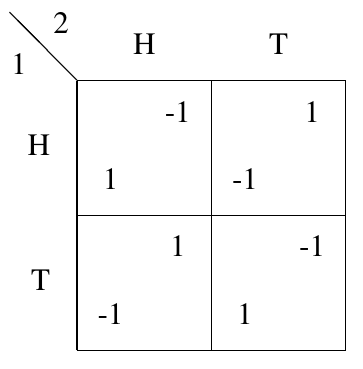
\includegraphics[width=.3\textwidth]{../img/matching-pennies.png}
      \caption[Matching Pennies]{Matching Pennies: player~$1$ as the Matcher, player~$2$ as the Mismatcher}
      \label{fig:matching-pennies}
    \end{figure}

  \item [Traffic Light]
    Two players, drivers of~cars, arrive at~a~crossroad perpendicularly to one another.
    If at most 1~driver crosses, the situation will be safe and their payoffs will be non-negative, with a~slightly better payoff for the passing player.
    If however both drivers decide to pass the crossroad, the result will be extremely sub-optimal, as both drivers obtain drastically negative payoffs and~die.

    \begin{figure}[H]
      \centering
      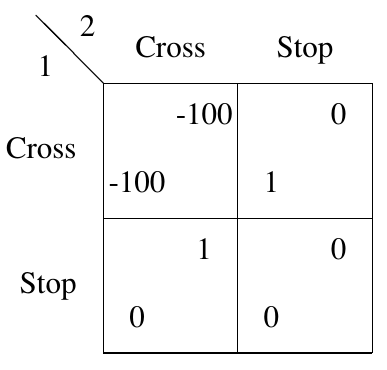
\includegraphics[width=.23\paperwidth]{../img/traffic-light.png}
      \caption{Traffic Light}
      \label{fig:traffic-light}
    \end{figure}

    This is an~example of~a~\emph{coordination game}, where a~common trusted \emph{coordination device} is desirable.
    Such a~device (e.g. a~traffic light or the right-of-way priority rule) justify the concept of~a~\emph{correlated equilibrium} (\cite[Subsection~1.3.6]{AGT07}).

  \item [Battle of Sexes] is another coordination game:
    Two players, Boy and Girl, are arranging an~activity for their date.
    The Girl wishes to go (S)hopping, while the Boy wants to go for a~(B)eer:
    \begin{figure}[H]
      \centering
      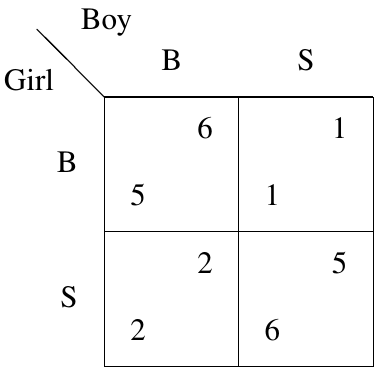
\includegraphics[width=.23\paperwidth]{../img/battle-of-sexes.png}
      \caption{Battle of Sexes}
      \label{fig:battle-of-sexes}
    \end{figure}
    Notice they both prefer to agree (rather than disagree) on~the activity, because this way they will be together.
    If however, they disagree and end up alone without a~date, both would rather spend the evening doing their favorite activity.
\end{description}

\begin{itemize}
  \item \emph{Prisoner's dilemma} \todo
    \begin{figure}[H]
      \centering
      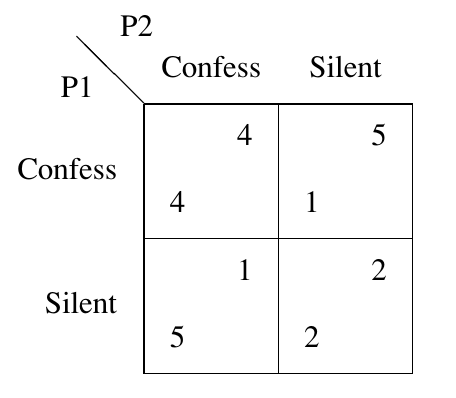
\includegraphics[width=\figurewidthratio\paperwidth]{../img/prisoner.png}
      \caption{Prisoner's dilemma}
      \label{fig:prisoner}
    \end{figure}

    \begin{figure}[H]
      \centering
      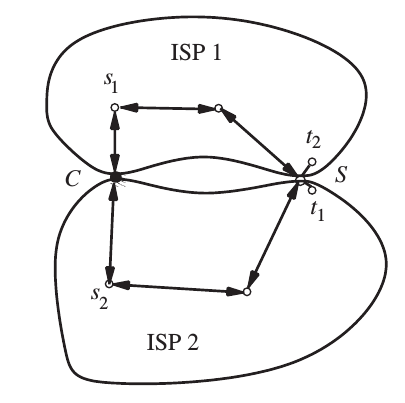
\includegraphics[width=\figurewidthratio\paperwidth]{../img/isp.png}
      \caption{ISP routing game}
      \label{fig:isp-routing}
    \end{figure}


  \item \emph{Pollution game} is a multi-player version of Prisoner's dilemma \todo

  \item Another coordination game is the \emph{Routing congestion game}, taken from the world of networking

    \begin{figure}[H]
      \centering
      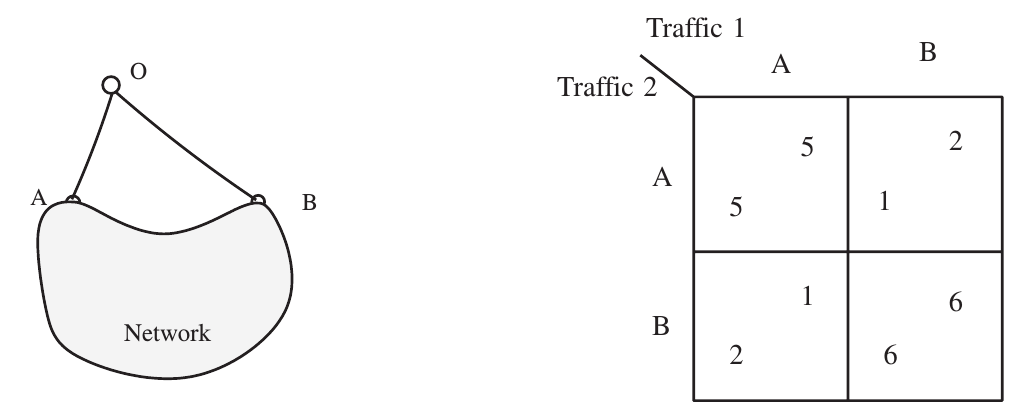
\includegraphics[width=0.65\paperwidth]{../img/routing-congestion-game.png}
      \caption{Routing congestion game}
      \label{fig:routing-congestion}
    \end{figure}

  \item \emph{Pricing game} is an~example of a~game without a~(mixed) \acrshort{ne}.

    \begin{figure}[H]
      \centering
      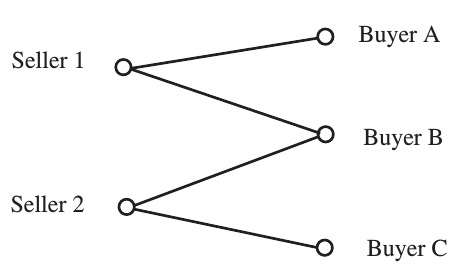
\includegraphics[width=\figurewidthratio\paperwidth]{../img/pricing-game.png}
      \caption{Pricing game}
      \label{fig:pricing-game}
    \end{figure}

  \item \emph{Ultimatum game}
\end{itemize}

\section{The Game of Go}
\label{sec:Go}

\subsection{Rules}

\emph{Black} and \emph{White} place pieces (\emph{stones}) on the unoccupied intersections (\emph{points}) of a~\emph{board} with a~$19\times19$ grid of~lines.
Players take turns, Black moves first.
There are only 2 basic rules of Go:
\begin{description}
  \item [The rule of liberty]
    Every stone remaining on the board must have at least one open point (an~intersection, called a~\emph{liberty}) directly next to it (up, down, left, or right), or must be part of a~connected group that has at least one such liberty next to it.
    \begin{figure}[H]
      \centering
      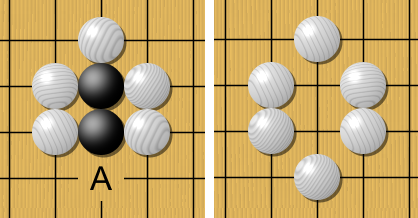
\includegraphics[width=.5\textwidth]{../img/Go_rule_of_liberty.png}
      \caption{The rule of liberty}
      \label{fig:Go-rule-liberty}
    \end{figure}

    Stones or groups of stones which lose their last liberty are removed from the board.

  \item [The ``ko'' rule]
    The stones on the board must never repeat a~previous position of~stones.
    This is to prevent unending cycles.
    \begin{figure}[H]
      \centering
      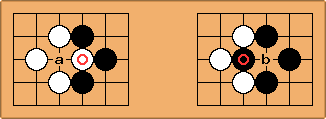
\includegraphics[width=.5\textwidth]{../img/Go_ko_rule.png}
      \caption{The ``ko'' rule}
      \label{fig:Go-Ko-rule}
    \end{figure}

\end{description}

\subsection{Scoring, Ranks and Handicaps}

There are several \textbf{scoring rules} to determine the winner of a~game.
In the match of~AlphaGo against Lee Sedol,%
\footnote{See Chapter~\ref{ch:AlphaGo}.}
the \emph{area scoring} was used.
Under area scoring system, player's score is:
\begin{itemize}
  \item the number of stones that the player has on the board
  \item plus the number of~empty intersections surrounded by that player's stones
  \item plus \emph{komi(dashi)} points%
    \footnote{a~compensation for the first move advantage of~the Black player}
    for the White player
\end{itemize}

\emph{Elo rating} can be used to denote players' \textbf{ranks}.
Alternatively, \emph{kyu/dan} (in~Japanese) or \emph{gup/dan} (in~Korean) system is also vastly popular:
\begin{figure}[H]
  \centering
  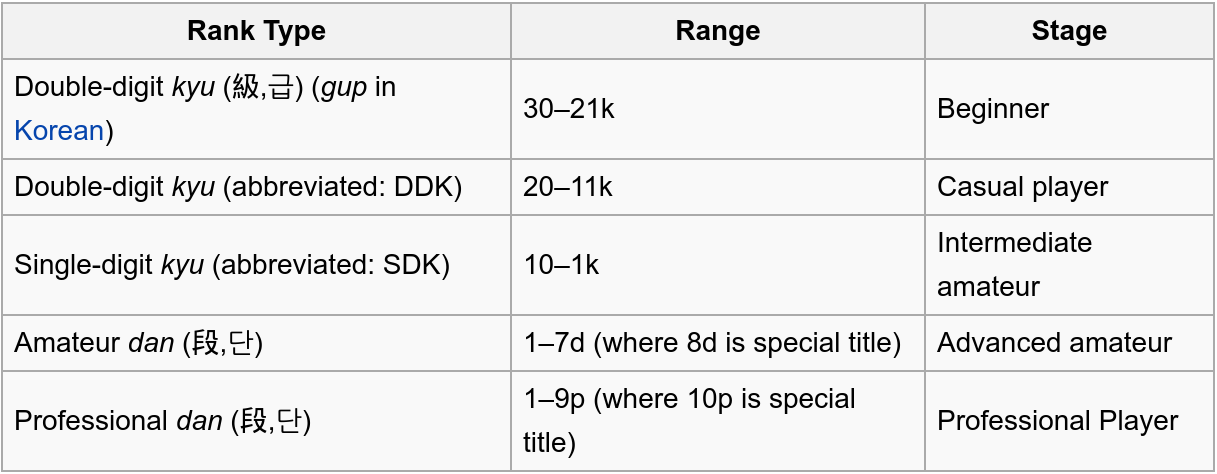
\includegraphics[width=.8\textwidth]{../img/Go_kyu_dan.png}
  \caption{Kyu/Gup and Dan ranks}
  \label{fig:Go-ranks}
\end{figure}

\textbf{Handicap} system is used to even up differences in ranks:
Black can place 1 or more stones in advance as a~compensation for White's greater strength.

\section{Combinatorial Game Theory}
\label{sec:CGT}
\todo

